% This must be in the first 5 lines to tell arXiv to use pdfLaTeX, which is strongly recommended.
\pdfoutput=1
% In particular, the hyperref package requires pdfLaTeX in order to break URLs across lines.

\documentclass[11pt]{article}

% Remove the "review" option to generate the final version.
\usepackage[review]{emnlp2021}

% Standard package includes
\usepackage{times}
\usepackage{latexsym}

% For proper rendering and hyphenation of words containing Latin characters (including in bib files)
\usepackage[T1]{fontenc}
% For Vietnamese characters
% \usepackage[T5]{fontenc}
% See https://www.latex-project.org/help/documentation/encguide.pdf for other character sets

% This assumes your files are encoded as UTF8
\usepackage[utf8]{inputenc}

% This is not strictly necessary, and may be commented out,
% but it will improve the layout of the manuscript,
% and will typically save some space.
\usepackage{microtype}


\usepackage{enumitem}

\usepackage{wrapfig}
\usepackage{hyperref}
\usepackage{graphicx}
\usepackage{multirow}
\usepackage{hyperref}
\usepackage{tabularx}
\usepackage{bm}
\usepackage{seqsplit}
\usepackage{xcolor}
\usepackage{stmaryrd}
\usepackage{booktabs}
\usepackage{fixltx2e}
\usepackage{xparse}
\usepackage{amsmath}
% \usepackage[dvipsnames]{xcolor}

\usepackage{multirow}% http://ctan.org/pkg/multirow

\DeclareGraphicsExtensions{.png,.pdf}
\label{packs}
% If the title and author information does not fit in the area allocated, uncomment the following
%
%\setlength\titlebox{<dim>}
%
% and set <dim> to something 5cm or larger.

%



\NewDocumentCommand{\heng}{ mO{} }{\textcolor{red}{\textsuperscript{\textit{Heng}}\textsf{\textbf{\small[#1]}}}}


\NewDocumentCommand{\chenkai}{ mO{} }{\textcolor{blue}{\textsuperscript{\textit{Chenkai}}\textsf{\textbf{\small[#1]}}}}


\NewDocumentCommand{\cheng}{ mO{} }{\textcolor{purple}{\textsuperscript{\textit{Cheng}}\textsf{\textbf{\small[#1]}}}}


\NewDocumentCommand{\bluetext}{mO{}}{\textcolor{blue}{#1}}


\title{Fine-Grained Chemical Entity Typing with Multimodal Knowledge Representation}
%Chenkai Sun, Heng Ji, Chengxiang Zhai

% Author information can be set in various styles:
% For several authors from the same institution:
% \author{Author 1 \and ... \and Author n \\
%         Address line \\ ... \\ Address line}
% if the names do not fit well on one line use
%         Author 1 \\ {\bf Author 2} \\ ... \\ {\bf Author n} \\
% For authors from different institutions:
% \author{Author 1 \\ Address line \\  ... \\ Address line
%         \And  ... \And
%         Author n \\ Address line \\ ... \\ Address line}
% To start a seperate ``row'' of authors use \AND, as in
% \author{Author 1 \\ Address line \\  ... \\ Address line
%         \AND
%         Author 2 \\ Address line \\ ... \\ Address line \And
%         Author 3 \\ Address line \\ ... \\ Address line}

\author{First Author \\
  Affiliation / Address line 1 \\
  Affiliation / Address line 2 \\
  Affiliation / Address line 3 \\
  \texttt{email@domain} \\\And
  Second Author \\
  Affiliation / Address line 1 \\
  Affiliation / Address line 2 \\
  Affiliation / Address line 3 \\
  \texttt{email@domain} \\}

\begin{document}
\maketitle


\begin{abstract}


% Unlike news, the scientific text usually requires domain expertise to understand. In recent years, NLP methods have leveraged domain expertise to improve the quality of IE on biomedical texts with huge impact.

% Unlike news, scientific text often requires multimodal domain expertise to understand, such as molecule knowledge for chemistry text. While Natural Language Processing methods have leveraged domain knowledge to improve the quality of Information Extraction on biomedical texts with huge impact, little work has been done in core chemistry literature, which forms the foundation of many biomedical research. In this work, we give a thrust to this underexplored yet important domain by introducing CHEMET, a benchmark dataset in fine-grained entity typing, and an effective method that incorporates external multimodal knowledge. Throughout our experiments, we showed that our method outperforms the state-of-the-art models in entity typing. To the best of our knowledge, this is the first work on tackling the problem of fine-grained chemical entity typing.

How to extract knowledge about chemical reactions from the core chemistry literature is a new emerging challenge that has not been well studied. In this paper, we introduce a new benchmark data set (CHEMET) to facilitate the study of knowledge extraction in this new domain. Fine-grained chemical entity typing poses interesting new challenges especially because of the complex name mentions frequently occurring in chemistry literature and graphic representation of entities. At the same time, there are also interesting new opportunities to leverage external chemistry knowledge resources. We propose a novel multi-modal representation learning framework to solve the problem of fine-grained chemical entity typing by leveraging external resources with chemical structures and using cross-modal attention to learn effective representation of text in the chemistry domain. Experiment results show that the proposed framework outperforms multiple state of the art. 



% ... or show that the proposed framework can effectively exploit external knowledge to improve accuracy of entity typing...

% Information extraction in scientific text is vastly different from news due to the amount of need for domain knowledge. While there was a surge of information extraction works on biomedical text in the past few years, 

% Information e xtraction refers to the task of transforming text into structured knowledge elements, which is a crucial step for many downstream tasks, such as knowledge graph construction and question answering. As the amount of research literature is growing exponentially, 
% Chemistry information e

% Compared to the news domain, information
% extraction (IE) from biomedical text requires
% much broader domain knowledge. However,
% many previous IE methods do not utilize
% any external knowledge during inference. Due


% This document is a supplement to the general instructions for *ACL authors. It contains instructions for using the \LaTeX{} style files for EMNLP 2021. 
% The document itself conforms to its own specifications, and is therefore an example of what your manuscript should look like.
% These instructions should be used both for papers submitted for review and for final versions of accepted papers.
\end{abstract}






\noindent\chenkai{colored sentences were added/modified/highlighted according to comments}


% \begin{figure*}
% 	\begin{center}
% 		\centerline{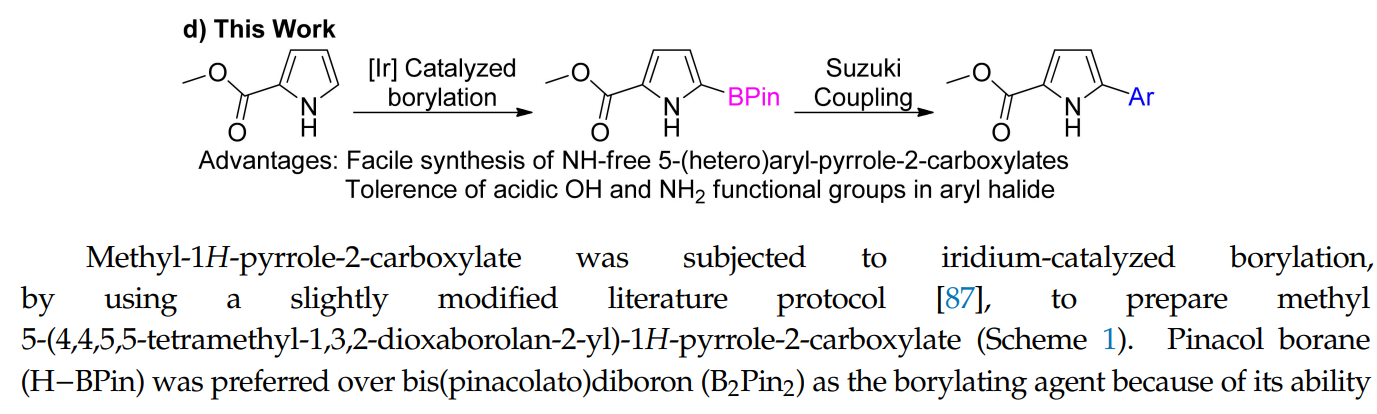
\includegraphics[width=2
% 			\columnwidth]{screenshot.png}}
% 		\caption{An screenshot of a portion of chemistry article~\cite{chem_article}. The text involves chemical formula, reaction, and complex chemical names.}
% 		\label{fig:screenshot}
% 	\end{center}
%  	\vskip -0.2in
% \end{figure*}

\section{Introduction}
\label{intro}
%\cite{abdalla-teufel-2006-bootstrapping}

% \heng{1.emphasize there is little NLP work for Chemistry domain; you propose a novel problem formulation and a potential solution; 2. walk through some examples when explaining the characteristics; 3. explain the main challenges to discuss the difference between Biomedical and chemistry domains; 4. distant supervision for training data acquisition; 5. for the walk-through example try to }

% \heng{only use 'work' instead of 'works', and use present tense instead of past tense}
% \heng{Explain why fine-grained entity typing is important for this domain, and what it is by giving a challenging example at teh beginning. } \cheng{I agree that a specific example at the very beginning would be very useful. We can use the example to make all the major (general) points we want to make. Perhaps a sample text, chemical structure and a target concept in an ontology?}
%Information extraction refers to the task of transforming text into structured knowledge elements, which is a crucial step for many downstream tasks, such as %knowledge graph construction and 
%question answering. 
As the amount of research literature is growing exponentially, accurate and efficient information extraction (IE) methods are crucial for many downstream applications including question answering and knowledge reasoning. One  domain largely overlooked by previous IE research is Chemistry (an example sentence is shown in Figure~\ref{fig:framework}), which consists of discussion on chemicals and reactions they are involved. What benefit can it bring if we develop well-performing IE methods for chemistry domain? If a comprehensive chemistry knowledge base can be efficiently constructed, chemicals can be discovered at a faster pace since models can learn from existing reactions to infer never-imagined ones, thus benefiting downstream applications such as those in biomedical research and chemical industry.  
% (a screenshot of a chemistry paper is shown in Figure~\ref{fig:screenshot})
%indispensable for structurizing text automatically in order to enrich knowledge base, which many inference tasks that require reasoning depend on. 
% COMMENTS
% \heng{simply say domain knowledge is too vague, need to elaborate it clearly: multi-modal representation, external knowledge via entity linking}

One fundamental building-block of information extraction is fine-grained entity typing (FET), which is the task of classifying entity mentions into subset of pre-defined hierarchical classes (e.g., Person/Artist, Location/City in news domain), and doing well in such task typically requires the system to understand the mention and its context well.
The task is particularly challenging for scientific articles, where domain-specific knowledge is heavily required to understand the text; for instance, in chemistry, one needs to understand the reaction mechanism in the literature described by both equation image and text (about experiment conditions), and since a reaction is based upon chemical compounds, it additionally assumes one to have knowledge about the chemical as well. Intuitively, to understand scientific articles, linking entities appearing in the text to retrieve and comprehend external information in different modalities would be very helpful. Analogically, when a person learns a cooking recipe, he or she would look up cooking instruction video (consisting of image, text, and audio) to help understanding the procedure In scientific domains, information extraction models have been widely developed for biomedical context~\cite{biomedie, biomedpp1, biomedpp2, biomedpp3, biomedpp4, scibert,biobert, biomedpp5,biomedpp6}  However, while chemistry research shapes the foundation of many biomedical studies, there has been little work done in extracting knowledge from core chemistry research literature; previous work in Chemistry IE mainly focuses on Named Entity Recognition (NER) (e.g., recognizing chemical name spans), and there is only one work we were able to find~\cite{chemu} on task other than NER (e.g., reaction event extraction). One major difference between chemistry and biomedical literature text lies in different chemical entity expressions, where chemical compounds in biomedical text are often expressed in natural language (e.g., water, aspirin), while in chemistry it's often complex formula-like names (e.g., 5,6-dihydroxycyclohexa-1,3-diene-1-carboxylic acid, H2O), which is hard to be understood by existing language models as such complex names do not follow morphological structure like other commonly used words like ``basketball''. To make the situation worse, many chemicals simply have never been coined with any nomenclature in natural language. The chemical mentions are essentially rare terms that is not best to be  and thus would be not learned well by language model  

%COMMENT
%  \heng{add more recent citations}

% Even if we pre-trained on these complex synonyms, most chemical entities would still be 

% COMMENTS
% \cheng{this point could be moved earlier to stress the importance of IE for chemistry domain. Perhaps we can first motivate IE in the literature in general and then say IE for Chemistry is especially important for reasons of xx, yy? Logically, it seems natural to first motivate the general problem of IE, then motivate the entity typing in general, and finally fine-grained typing. We can then discuss the unique challenges of fine-grained typing that make existing approaches to typing inadequate. We propose to use multimodal knowledge representation to address the (unique) challenges. In the experiment part, we can then show the proposed approach is indeed effective for addressing the new challenges (e.g., by showing cases where SOTA methods failed, but the proposed approach succeeded.}
%, thus benefiting different parties, including biomedical studies and chemical industries.
% In this work, we explore fine-grained chemical typing, which is the task of classifying chemical mentions into fined-grained types. 
% COMMENTS
% \cheng{Need to briefly mention existing methods to entity-typing here and why they may be inadequate for the chemical fine-grained typing. Is it because of the challenge associated with Chemistry or the ``fine-grained" typing. In general, it might be good to say something like "Our (new) task poses several (unique/new?) challenges: (a) Chemsitry domain... (b) fine-grained (vs. coarse grained)..... It would be great to clarify which is the major challenge that we focus on tackling. } 


% COMMENTS
% \cheng{Is it possible to coin a new name for ``this promising field"? Or otherwise be specific, e.g.,  ``Chemical Information Extraction"? Is this term already standard? Or perhaps "Chemical Knowledge Base Population"? }
Although there has been a line of method in FET applied to news domain~\cite{ultrafet, label_bias, fet_el, lin2019attentive,hierarchical_gcn, hyperbolic}, none have been developed for core chemistry literature and they do not consider any types of domain-specific knowledge. While language model may have a hard time understand the chemical mention purely based on its surface form and contextual representation, we can understand the identity through it's external information (in different modalities) such as natural language description about its properties and it's structure (or graph). In the chemical typing task particularly, compound types can be well correlated with properties and physical structure 
% COMMENTS

% \heng{use this to motivate why text-only representation is not enough}  
%in chemical literature, which potentially improves the understanding of chemical mention and learn correlation between different entities.
% , we see the urgent need of a line of benchmark datasets and methods to encourage people to drive this promising field, \bluetext{Chemistry Information Extraction (ChemIE)}.
% While general domain language model can be massively pre-trained upon external text to achieve a good performance in chemical entity classification, they miss incorporate different modalities of information, such as chemical structures. 

% COMMENTS

% \heng{need to emphasize the novelty of the work: multimodal information, incorporating external knowledge}
% \cheng{it would also be good to discuss the generality of the novelty. Is the novelty specific to the particular problem/task or Chemical domain? Or perhaps it's novel in the context of typing? Clarifying the scope of novelty would be helpful. It can either help ``defend" the novelty if it's only specific to Chem IE, or help ``amplify" the novelty/impact if it's not just restricted to Chem IE.} 
% \heng{for paper writing, use present tense instead of past tense for both of your work and related work}
Our work is novel in that we are the very pioneers to explore FET strategies in chemistry. Utilizing external database for multimodal information retrieval, we introduce a deep learning based method that use cross-modal attention to align and embed the structure and description text of chemicals into a common space as core features for classification. %, which under the shell aims to align properties phrase and molecule substructure.
As illustrated in Figure~\ref{fig:intuition}, %intuitively,
some patterns of molecular substructures well align with the phrases in description text. For example the circled sub-structure in the is commonly appeared together with  "polar aprotic".

% comment
% \heng{I commented out the following sentence because it's very confusing, need to re-write:}

%The addition of multiple modalities targets achieving the same goal as image-text co-embedding, that is, to build a unified representation that allows reasoning over different perceptions; such representation can result in more discriminative predictions, which is shown in our experiments.


% comment

% \cheng{"limited dataset" is a bit vague. I think we can say more definitely that there doesn't already exist such a data set, right? I'm thinking of something like ``Since the proposed task has not been studied in the previous work, there is no dataset available for evaluating the task. To facilitate the study of this new task, we construct the first data set for fine-grained typing in the chemistry literature domain..... .}
Since the proposed task has not been studied in the previous work, there is no dataset available for evaluating the task. To facilitate the study of this new task, we construct CHEMET\footnote{Both the dataset and the code will be released to public}, the first dataset for fine-grained typing in the chemistry literature domain, for which we referred to wikipedia category for ontology construction, and used distant supervision to generate training data and facilitate annotation procedure. The dataset was based upon a corpus of 50 open access papers from a database on a specific theme. We will discuss the data construction details in Section \ref{datacollection}. Experimental results on the the dataset show that our method outperforms the state-of-the-art methods in entity typing. To the best of our knowledge, our method is the first to take step toward tackling fine-grained chemical entity typing.

% Since there is no dataset available for chemical FET, we have collected and annotated a new dataset, 

%  We will release the dataset in our code repository. 

Overall, our contributions can be summarized as the following:
% comment

% \heng{convert these into bullets} 
% \heng{the following bullets need to be re-written in a more concise and formal way}


\begin{itemize}
    \item We study the task of fine-grained chemical entity typing in chemistry literature, a largely under-explored yet promising field for NLP that has a great need for information extraction methods
    \item We construct the first human-annotated dataset in  fine-grained chemical entity typing and will release to the public.
    \item We introduce an novel method that utilizing multimodal knowledge representation to enrich entity mention representation
    \item The multimodal component of the model is based on structure and text alignment, which has never been explored before and can be applied to variety of ChemIE tasks such as relation extraction and event extraction.
    \item Experiments on the dataset show that our model outperforms the state-of-the-arts entity typing models. 
\end{itemize}




% that has a great needs information extraction methods in order to conduct experiments more efficiently

% \st{In this work, we explored relation extraction, the task of classifying 
%relationship between named entities (given by the task) into a subset of 
%predefined classes. Since there is no existing chemical benchmark on 
%information extraction, we also release a  dataset on named entity 
%recognition, 
%relation extraction, and event extraction, based on chemistry research 
%articles 
%on diverse topics. The ontology was carefully crafted in collaboration with 
%chemistry authorities, and data samples are annotated by chemistry students. 
%The dataset was designed in hope of encouraging further development of 
%information extraction methods on chemistry literature. In short, we made the 
%following contributions:...}





\begin{figure}
 	\vskip 0.2in
	\begin{center}
		\centerline{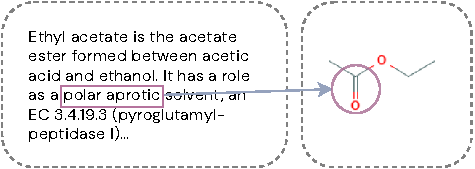
\includegraphics[width=0.9 
			\columnwidth]{intuition.pdf}}
		\caption{An example of chemical entity structure aligning with textual concepts. The circled sub-structure is
		often induce the "polar aprotic" property
% 		commonly described by polar aprotic"
		infer that ethyl acetate is polar aprotic}
		\label{fig:intuition}
	\end{center}
 	\vskip -0.2in
\end{figure}



\begin{table}
	\caption{Dataset Statistics for CHEMET}
	\centering
	\begin{tabular}{lllll}
		
		\toprule
		Setting &Anno.& \#Inst. & \#Mention  & \#Types \\
		\midrule
		Train &Distant&   8000& NA&43\\
		Dev &Human&1000&NA&NA\\
		Test&Human&            1000&NA&NA \\
		\bottomrule
	\end{tabular}
	\label{datastats}
\end{table}



\begin{figure*}[ht]
% 	\vskip 0.2in
	\begin{center}
		\centerline{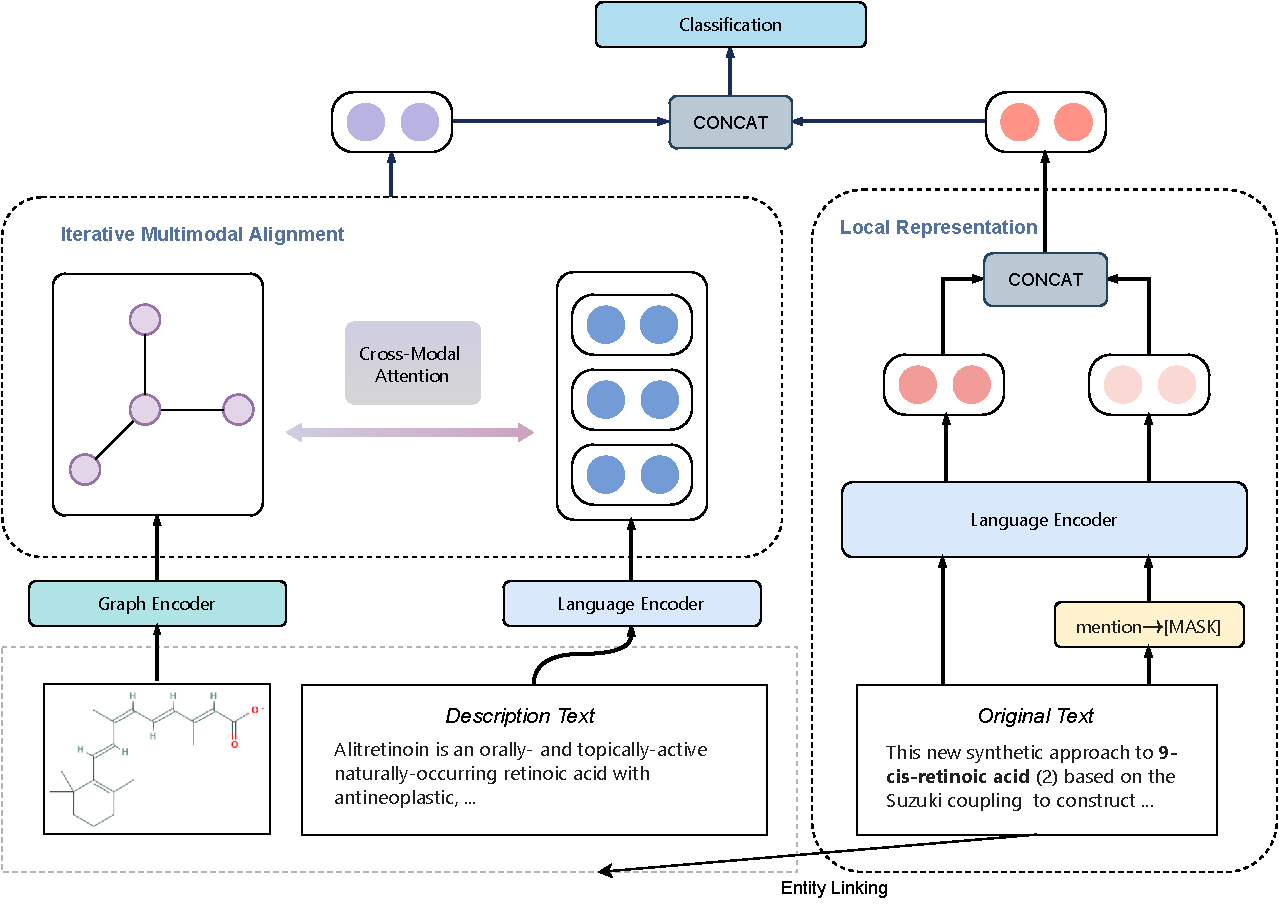
\includegraphics[width=2
			\columnwidth]{model_new.pdf}}
		\caption{Our fine-grained chemical entity typing model architecture. Please refer to Section~\ref{sec:method} for details. \heng{1. label "KB" and "Literature"; 2. make font bigger. }
		}
		\label{fig:framework}
	\end{center}
	\vskip -0.2in
\end{figure*}
\section{Dataset}
%\subsection{Data Collection}
\label{datacollection}

% Krippendorff alpha, or other 
% agreement metric

% describe diversity

\cheng{"limited dataset" is a bit vague. Is there any such data set available? If so, we should try to use it. My sense is that there isn't(?), so the novelty and significance of the data set could be more clearly articulated.}
\bluetext{Since there is no dataset available for fined-grained chemical entity typing, we have collected and annotated a dataset, CHEMET, based on a corpus of 100 papers from PubChem) with Suzuki-Coupling (a popular reaction mechanism) theme; the theme was chosen to align with chemistry annotators' domain knowledge. We will discuss the steps taken to construct the dataset below.}

\noindent \textbf{Taxonomy Construction}. \cheng{how was the number xx determined? try to give a justification or explanation of the process that reached the number xx. }\bluetext{In taxonomy construction, we focus on collecting the types that belong to chemicals commonly occurring in Suzuki-Coupling literature. We carefully select sub-categories from wikipedia chemistry category page~\footnote{\url{https://en.wikipedia.org/wiki/Category:Chemistry}} as fine-grained ontology; for example, Organic chemistry$\rightarrow$Organic compounds$\rightarrow$Esters is a fined-grained type where right of the arrow is the sub-category of the left. The ontology is shown in Appendix~\ref{sec:appendix1}}
% \cheng{The following sentence can be moved earlier in this paragraph to explain the strategy being taken. It's better to first give a description of our goal/strategy/philosophy and then describe how we do it. If there are decisions to be made, explain why we've decided to choose one options not another.} 

\noindent \textbf{Distant Supervision} 

% In order to ease human annotators' work and to collect training data, we employed distant supervision to retrieve noisy labels for the corpus. In this step we first tokenized text using~\cite{oscar4}, a texting mining framework for chemistry that recognize complex chemical name well. We then collected a dictionary mapping from picked types (that is, the select categories from Wikipedia) to their belonging wikipedia pages. We treated the page titles as entity names. Since a compound can have many synonyms, we queried PubChem to expand the dictionary. Finally, we used the dictionary to label the tokenized text using a well-performing string matching algorithm.
\cheng{Provide a reference to this string matching algorithm or elaborate.}

\jinfeng{I'm re-writing this section as below. Free free to use any part of it.}

We employed distant supervision from Wikipedia and PubChem to create noisy entity labels for the corpus. This process involves the following steps. 1) We first populated entities into the nodes (i.e., entity types) of the taxonomy. That generated an \textit{entity dictionary}. More details are given in the next paragraph. 2) We then tokenized the corpus using~\cite{oscar4}, a texting mining framework for chemistry that recognizes complex chemical name well. 3) Finally, we distantly labeled the corpus with the entity dictionary by following the procedure of training data generation in AutoNER \cite{DBLP:conf/emnlp/ShangLGRR018}.

Now we give more detailed description of our process of automatically assigning entities to types. Each type (except those starting with ``Other'') is a node in our taxonomy that corresponds to a category in Wikipedia. Each category can have sub-categories and associated pages. Starting from each type, we traced its sub-categories recursively by performing a depth-first search (DFS) with a maximum depth of three. In the DFS we skipped those sub-categories that are probably irrelevant to Chemistry. We used a spell-checker dictionary \cite{azman2012chemistry} with over 104,000 technical chemistry terms, and dropped a category from the search if less than 20\% of the 1-grams in its name and the names of all its direct children were covered by the dictionary. The maximum depth of three and threshold of 20\% were selected empirically by manually checking the quality of the results for some types. After the DFS, we populated the Wikipedia page titles associated with any sub-category of a type as entities of that type. For each type starting with ``Other'', we took the difference between the entities assigned to its direct parent category and those assigned to all its siblings as its entity list. Finally, we expanded each entity with its synonyms from the PubChem database\footnote{https://ftp.ncbi.nlm.nih.gov/pubchem/Compound/Extras/CID-Synonym-filtered.gz}.

\noindent \textbf{Human Annotation}.
Note: talk about agreement metric

% Note: talk about diversity

We hired five undergraduate chemistry students as annotators. The annotators were instructed to identify and type spans in the assigned samples using Brat~\cite{brat} interface. To ensure the diversity of the testing data, we randomly select the test samples from the corpus for annotation. In order to mitigate annotator bias, we distributed each sentence to three annotators, and take majority vote from the results. The dataset statistics is shown in Table~\ref{datastats}.


%\subsection{Data Analysis}

%\label{dataanalyze}
%\noindent \textbf{Size}. 
%
%\noindent \textbf{Entity Types}. 


\section{Method}
\label{sec:method}
% \cheng{Before describing the method, it's better to briefly motivate the method. Perhaps remind the readers what are the key (new) challenges we need to address, and then briefly describe the proposed ideas for addressing those challenges informally. This would help readers see the big picture (in terms of novelty and justification) before going over the detail of the model.}
\bluetext{Chemistry literature is unique in that the mentions are often expressed in complex, unnatural forms, as shown in the snippet in Figure~\ref{fig:framework}. At the same time, external databases contains multimedia definition about chemical entity, such as chemical structure and natural language description. It is thus a natural idea to incorporate these different forms of representation of an entity to enhance the system's understanding on a chemicals. In our methodology, we develop an effective deep learning based model to implement such idea.}

The overall model architecture is presented in Figure~\ref{fig:framework}. Given a sentence $S$ marked with mentions, we first extract external information (chemical structure and natural language description) by linking to PubChem, one of the mostly used chemical database; we use its search API to fetch entity information given a mention name. We also used a modified version of $S$ that mask the entire mention name, to combat the issue of complex chemical name (\ref{sec:context}). We then proceed to extract features from local context and from external multimodal definition. The multimodal features are passed through cross-attention stage (\ref{sec:cmsa}) to learn a unified representation. Finally we use all features learned to classify the mention.

%for instance, graph neural network for structure input and Pretrained Language Model for 



\subsection{Original Text Embedding}
\label{sec:context}

Given the original sentence $S$, we first insert a marker symbol ``*'' at the start and end of the mention $m$ during preprocessing, following~\cite{atlop}; similar approach is also used in \cite{marker1, marker2}. The model first encodes the original sentence with SciBERT~\cite{scibert}, a Transformer~\cite{transformer} based language model pre-trained on biomedical text. Let $T=[t_1, t_2, ..., t_z]$ be the tokens in $S$ after tokenization (we implicitly assume the presence of [CLS] and [SEP] tokens and omit them from for cleanness), where $z$ is the number of tokens. Then we pass the tokens into SciBERT to to obtain contextual representations:
\begin{equation}
[\mathbf{t}_1, \mathbf{t}_2, ..., \mathbf{t}_z]=\text{SciBERT}([t_1, t_2, ..., t_z])\end{equation}

\noindent Where $\mathbf{T}=[\mathbf{t}_1, \mathbf{t}_2, ..., \mathbf{t}_z] \in \mathbb{R}^d$ and $d$ is the
number of hidden dimensions. We then use the embedding of ``*'' before $m$ as the mention embedding. Let us denote the mention embedding as $\mathbf{m}$.

% Then we follow \cite{e2ecoref} and compute the representation for mention $m$ by $$\mathbf{m}=\text{FFNN}_t([\mathbf{t}_{\text{START}(m)}, \mathbf{t}_{\text{END}(m)}, \hat t, \phi{(m)}])$$, where $\text{FFNN}_t$ is a feed forward neural network. $\text{END}(m)$ and $\text{START}(m)$ denote start and end indices for $m$. $\hat t$ is the representation based on attention to each token in $m$. 

%The $\text{FFNN}$ below will be the same.

\subsubsection{Context-only Embedding}
Since chemical entities often involve complex names that are difficult to be understood, we also produce a representation that rely less on the word structure of the mention, since the mention often not follows morphology (e.g., [3H]MK-801, NSC-406186, 8-azido-[alpha-32P]ATP). We first replace the entire span of mention by [MASK], then the modified sentence is embedded by SciBERT and the embedding for the [MASK] token is used as the corresponding context-only embedding for the mention, denoted $\mathbf{m}_\text{MASK}$. The context-focused embedding is then concatenated with mention embedding to represent local information, denoted by $\mathbf{m}_\text{L}=[\mathbf{m};\mathbf{m}_\text{MASK}]$.

\subsection{Multimodal Encoder}
\label{sec:cmsa}

% \chenkai{please ignore, whole thing will be changed}

As one of our core contributions, we propose to incorporate multimodal definition to expand chemical representation, and to combat the difficulty of understanding complex chemical mention name (e.g., (E)-3-(3,4-dihydroxyphenyl)prop-2-enoic acid) purely based on context and morphological structure. 

Specifically, we use API provided by PubChem as the entity linker to retrieve chemical structure and natural language description for each chemical mention. Chemical structure refers to a graph where bonds are edges and atoms are nodes, and description text discusses chemical properties (e.g., Aspirin is an orally administered non-steroidal antiinflammatory agent). 

% One another benefit is that system can implicitly learn to better cluster molecules even if a chemical entity is missing some modalities (e.g., only have structure available), since we map both modalities into the same embedding space.
To learn concepts from multiple modalities that better correlate with target label and to build more accurate representation of a molecule, we made use of the recently successful attention mechanism to co-embed concepts (or molecule property) in text and substructure in chemical graph in order to capture interaction between different modalities. 

Formally, let $G=(V,E)$ denote the chemical graph with $a$ nodes, and $D=[ d_1,d_2,...,d_b]$ denote the sequence of $b$ tokens after tokenizing description sentences. Similar to the embedding the sentence from literature, we embed the tokens with SciBERT  for which output is $\mathbf{D}=[\mathbf{d}_1,\mathbf{d}_2,...,\mathbf{d}_b]$. We also embed the nodes in chemical structure using Graph Isomorphism Network (with edge features)~\cite{gin}, a powerful graph neural network that can well capture different graph patterns. We randomly initialize embedding for each atom and bond type and use them to initialize node and edge embedding, and update node embeddings as below

\begin{equation}
\mathbf{n}_i^{l+1}=\text{FFNN}^{l+1}\bigg((1+\epsilon)\mathbf{n}_i^{l}+\sum_{j\in\mathcal{N}(i)}\mathbf{n}_j^{l}+\mathbf{e}^{l}_{j,i}\bigg)
\end{equation}
% _\theta^{(l+1)}
% \begin{equation}
% \begin{split}
% F = \{F_{x} \in  F_{c} &: (|S| > |C|) \\
%  &\quad \cap (\text{minPixels}  < |S| < \text{maxPixels}) \\
%  &\quad \cap (|S_{\text{conected}}| > |S| - \epsilon) \}
% \end{split}
% \end{equation}


\noindent where $\mathbf{n}_i^{l}\in \mathbb{R}^d$ is node representation for node $i$ at $l$-th layer, $\epsilon$ is a tuning hyperparameter, $\mathcal{N}(i)$ is the set of neighbours of node $i$, and FFNN is a feed forward neural network with two hidden layers (the first one maps from $\mathbb{R}^d$ to $\mathbb{R}^{2d}$ with Tanh activation, and the second one maps $\mathbb{R}^{2d}$ back to $\mathbb{R}^{d}$ without activation). We denote node representation $\mathbf{N}=[\mathbf{n}_1,\mathbf{n}_2,...,\mathbf{n}_a]$.


% \mathbf{n}_v^{(l+1)}=\text{MLP}_\theta^{(l+1)}\bigg((1+\epsilon)\mathbf{n}_v^{(l)}+\sum_{w\in\mathcal{N}(v)}\mathbf{n}_w^{(l)}+\mathbf{e}^{(l)}_{w,v}\bigg)


% d_{[CLS]}
We leverage self-attention mechanism of \cite{transformer} to learn dependency between different modalities. To achieve this, we first stack node and token embeddings as

\begin{equation}
\mathbf{X}=\begin{pmatrix}
\mathbf{N} \\
\mathbf{D}
\end{pmatrix}, \ \mathbf{X}\in\mathbb{R}^d
\end{equation}

\noindent where $\mathbf{X}\in\mathbb{R}^d$. Then the stacked embedding is passed through a Transformer layer to learn cross-modal association
\begin{equation}
[ \Tilde{\mathbf{n}}_1, \Tilde{\mathbf{n}}_2, ..., \Tilde{\mathbf{d}}_1, \Tilde{\mathbf{d}}_2...]=\text{Transformer}(\mathbf{X})\end{equation}

% Then we compute key values of the matrix by $\mathbf{Q}=\mathbf{X}\mathbf{W}^Q$,$\mathbf{K}=\mathbf{X}\mathbf{W}^K$, and $\mathbf{V}=\mathbf{X}\mathbf{W}^V$


% Then the attented representation is given by 

% $$\text{Attention}(\mathbf{Q},\mathbf{K},\mathbf{V})=\text{softmax}(\frac{\mathbf{Q}\mathbf{K}^T}{\sqrt{p_k}})\mathbf{V}$$

% where $\frac{1}{\sqrt{p_k}}$ is a scaling factor in \cite{transformer}. We used an average pooling to get multimodal representation $\mathbf{E}_{CM}$
\noindent and the cross-modal feature is then obtained by maxpooling the output from transformer layer

\begin{equation}
    \mathbf{f}_\text{cm}=\text{MaxPool}([ \Tilde{\mathbf{n}}_1, \Tilde{\mathbf{n}}_2, ..., \Tilde{\mathbf{d}}_1, \Tilde{\mathbf{d}}_2...])
\end{equation}


In addition, we preserve the unimodal graph representation by mean pooling over the node representation $\mathbf{N}$, to get $\mathbf{f}_{g}$. We also use the [CLS] token embedding $\mathbf{d}_{[CLS]}$ to represent unimodal text features. We then obtain a the multimodal definition vector

\begin{equation}
    \mathbf{f}=[\mathbf{f}_\text{cm};\mathbf{f}_{g};\mathbf{f}_{[CLS]}]
\end{equation}
\subsection{Final Prediction}

Let E denote the set of entity types. Lastly, we predict the final entity type by using features from both local context and multimodal information
\begin{equation}
\mathbf{p}=\text{Sigmoid}(\text{FFNN}([\mathbf{m}_\text{L};\mathbf{f}]))\end{equation}

\noindent where $\text{FFNN}$ is a feed forward neural network mapping from $\mathbb{R}^d$ to $\mathbb{R}^{|\text{E}|}$. $\mathbf{p}$ is the final probability distribution of classes.
% where $\mathbf{W}^f$ is a learnable weight matrix

\subsection{Training}
We use multi-label soft margin loss for training, that is,
\begin{equation}
\begin{split}
    \mathcal{L}=\frac{1}{C}\sum_{i=1}^{C}\Bigg( y_i\log\bigg(\frac{1}{1+e^{-x_i}}\bigg) +\\ (1-y_i)\log\bigg(\frac{e^{-x_i}}{1+e^{-x_i}}\bigg)\Bigg)
\end{split}
\end{equation}
\noindent In the equation, $C$ is number of classes, $y_i$ indicates true (binary) label for class $i$ and $x_i$ is the predicted probability for class $i$.



% as pointed out by~\cite{mmdl}, simple concatenate features from different modalities result in a shallow representation since the correlation, or interaction, between the modalities is highly non-linear.

%  it is important to
% learn joint embeddings to leverage the complementarity of
% multimodal data to represent such concepts more accurately

% to learn a more complete representation of the molucule, we need to ground the structure on textual propreties

% better
% features for one modality (e.g., video) can be
% learned if multiple modalities (e.g., audio and
% video) are present at feature learning time


% The flow of
% knowledge from one data modality to another is a challenging
% task.


% This allows for fast selection
% of a new trajectory by projecting a new environment/instruction pair and
% choosing its nearest-neighbor trajectory in this space.

% noise cancel
% so even only one part unreliable, can st infer , two similar compound similar label

% pick out important concepts that distinguish

% o perform reasoning with a variety of sensing modalities.

% unified repr

% Mapping to common space, so cancel noise
%  a shared embedding spac
% has the following advantages

% Although deep learning architectures do
% a good job of learning these vector representations in isolation, learning a single common representation across multiple
% modalities is a challenging task
% \begin{itemize}
%     \item It attends to important features in each modality, thus cancelling noise
%     \item Attention has proved its effectiveness in many visual and
% language tasks [23, 1, 7, 52, 50], it is designed to capture a
% better representation of image-sentence pairs based on their
% interactions.
% \end{itemize}




%After the above 
%Following~\cite{cmsa}, we also use self attention for encoding



% \subsection{Final Prediction}

% Concatenation, FFNN, Loss Function 
\begin{table*}[t]
	\caption{Transductive Imputation AUC with 10\% missing data}
	\centering
	\label{10perc}
\begin{small}
		
		\begin{sc}
		\begin{tabular}{llll}
			\toprule
			Model &                      Accuracy &                          
			Macro-F1 &                Macro-F1  \\
			\midrule
			1&1&1&1\\
			
			\bottomrule
		\end{tabular}
		
	\end{sc}
	\end{small}
\end{table*}

\section{Experiments}

Since there is no other fine-grained chemical entity typing datasets to our knowledge, we evaluate fine-grained chemical entity typing on the CHEMET. The experiments can be reproduced using implementations provided in supplement material.
\subsection{Baseline Methods}
\cheng{It would help to clarify what questions we can answer by comparing the proposed methods with these baselines. It seems to me that these baseline methods do NOT use the same amount of information/resources as the proposed method. If so, the improvement may have come from the fact that we have used additional information/resources, which wasn't used in the baseline methods. This wouldn't be a surprising finding as we are expected to do better with more resources/information. The more interesting question here is: what's the best way of exploiting such information? So if possible, it would be great to include stronger baseline methods that use the SAME amount of extra information. This would help showing the proposed  method is better, not just because it has access to more information/resources, but also because the method can better utilize the extra information than a baseline way of using it (e.g., straightforward combination of existing methods to achieve the goal). Ideally, the baseline methods can be aligned with the most relevant previous work discussed in the related work section. This would help us empirically examine/support the novelty of the work in comparison with previous work from multiple perspectives (e.g., the perspective of tackling the complex name mentions, the perspective of multi-modal attention/embedding, and the connection between local context with molecule structure(?). }
 In the experiment, we compared our method with the following state-of-the-art text classification and fine grained entity typing models,
%(NER) 

\noindent \textbf{SciBERT}. SciBert~\cite{scibert} is a Transformer based language model pretrained on sample of 1.14M papers from Semantic Scholar, in which 82\% are from the broad biomedical domain. A linear layer is applied on the embedding of $[$CLS$]$ for classification.

\noindent \textbf{BioBERT}. Similar to SciBert but pretrained on PubMed abstracts (PubMed) and PubMed Central full-text articles (PMC). Similar to SciBRET, a final linear layer is applied for classification.

\noindent \textbf{Latent Type Representation}. \citet{lin2019attentive} used a hybrid classification method beyond binary relevance to exploit type inter-dependency with latent type representation

\noindent \textbf{Fine-Grained Entity Typing in Hyperbolic Space
} Utilized hyperbolic embeddings. If have time.


%\noindent \textbf{Fine-Grained Entity Typing in Hyperbolic Space}. used Hyperbolic embedding



%\noindent \textbf{Baselines}.
%\noindent \textbf{Implementation}


\subsection{Implementation Detail}

follow Hyspa

<ModelName> was implemented using PyTorch \cite{pytorch} and Huggingface Transformers \cite{huggingface} with SciBERT as text encoder. We left model and training parameters and reproducibility details in the appendix for interested readers. 

\subsection{Result}

\subsection{Ablation Study}
To show the improvement made by each of the submodules in our method, we truncate model in the following way

\begin{itemize}[noitemsep,topsep=0pt]
	
	\item w/o multimodal alignment: FFNN
	\item w/o molecule graph: 
	\item w/o description text: 
\end{itemize}


\subsection{Attention Analysis for Structure-Text Alignment}
By the heatmap visualization

\subsection{Error Analysis}
Here we analyzed the remaining errors and categorize the into different cases  (shown in Figure \ref{error_dist}). We discuss the most common ones below

% \begin{figure*}[ht]
% 	\begin{center}
% 		\centerline{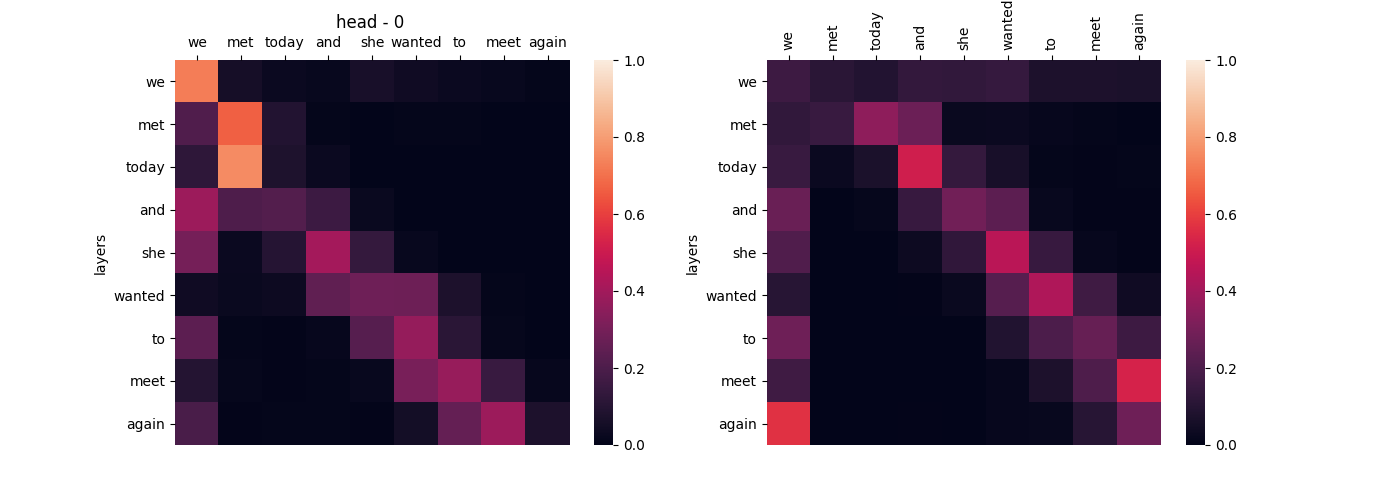
\includegraphics[width=1 
% 			\columnwidth]{attn.png}}
% 		\caption{Self Attention Framework}
% 		\label{fig:attn}
% 	\end{center}
% \end{figure*}

\begin{figure}[t]
	\centering
	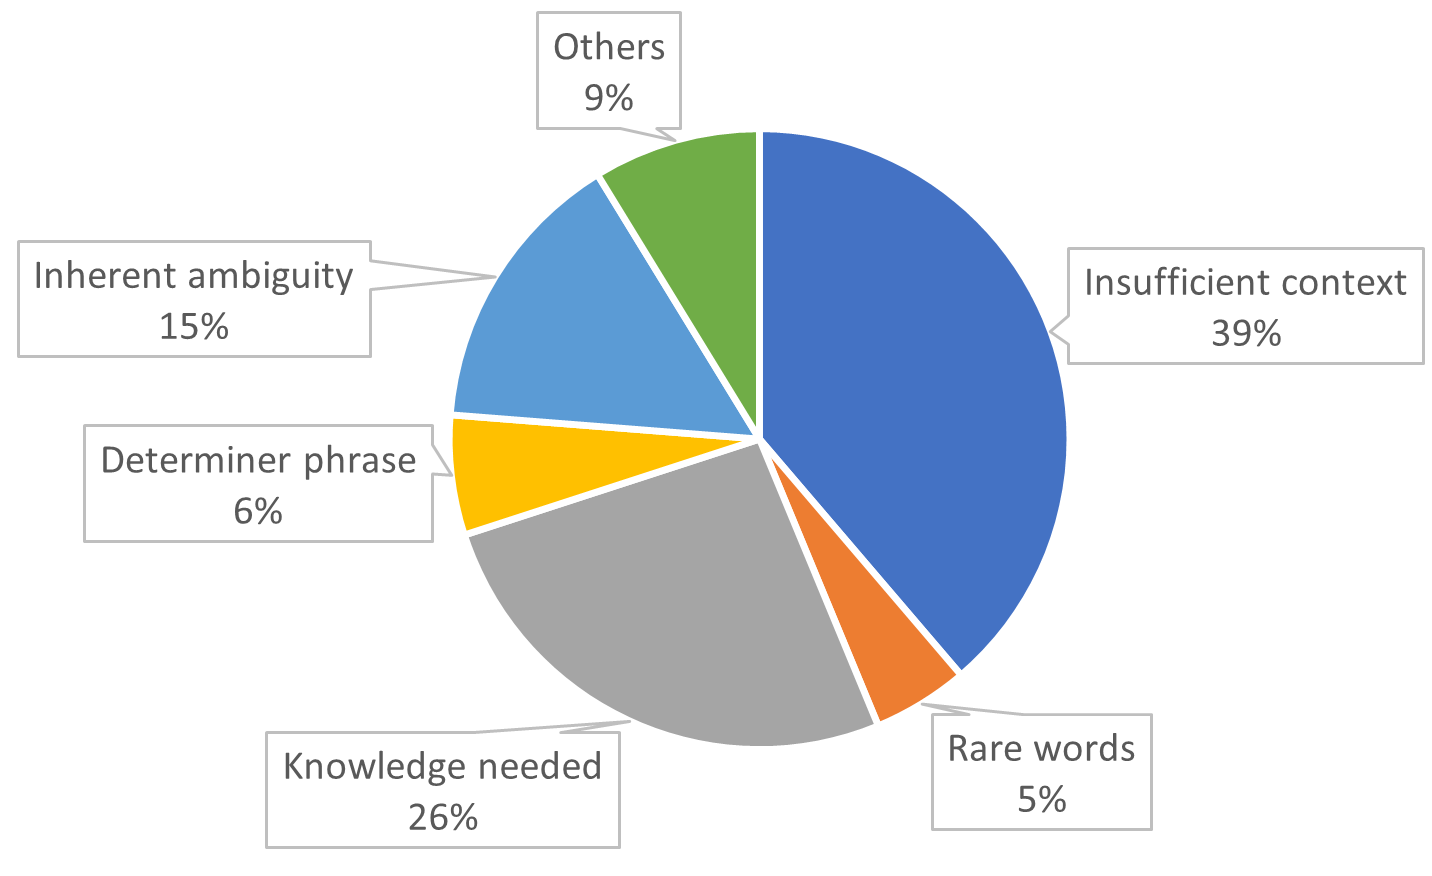
\includegraphics[width=0.9\columnwidth]{case_dist.png}
	\caption{Distribution of remaining errors on the test set.}
	\label{error_dist}
\end{figure}




\section{Related Work}
% The followings are relevant works for now.

% \subsection{Dataset Construct}
% \subsection{Scientific IE}

% \textbf{\textcolor{purple}{In progress}}


% \heng{add a subsection about the work using external knowledge to improve IE, such as Lai2021b and Zhang2021b}

\subsection{Fine-Grained Entity Typing}
There has been a wave of Fine-Grained Entity Typing (FET) methods in recent years~\cite{ultrafet, label_bias, fet_el, lin2019attentive,hierarchical_gcn, hyperbolic}. \citet{label_bias} propose to capture label correlation by employing graph convolution network on label co-occurrence matrix. \citet{fet_el} makes %, on the other hand, made 
use of an existing entity linker to obtain noisy external data in order to enrich and disambiguate mention representation. The authors also use entity linking scores as additional features. \citet{lin2019attentive} exploit type inter-dependency with latent type representation. Previous FET methods, however, only focused on news domain where text comes from news or wikipedia article and speech.  

% \heng{emphasize all of the previous work only focus on general news domain or wikipedia data}

% Chemistry text, however, is largely different from news in that it's not only heavy in domain-specific knowledge, but also often has complex mention names not following morphological structure (sometimes alphanumeric encoding). Up until now, there has been no dataset or work in chemical FET, which is important for mining compound entities from unstructured chemistry literature. We have not only built a new benchmark, but also developed an effective FET framework that incorporates external structure and text knowledge. \heng{not sure what you mean by 'external structural'?} \cheng{It seems that ``complex mention names" is a main new technical challenge. It would be great to amplify this message throughout the paper including a discussion of why the proposed model/architecture/framework can be expected to address this challenge and some empirical results to show the effectiveness in addressing the challenge (e.g., an example where previous methods failed to work because of the complex mention names but the proposed new method worked better. Another way to discuss the novelty here is to say the previous methods have NOT fully exploited the opportunity in our problem domain (e.g., external information/knowledge) and we propose a FET framework to enable full exploitation of external resources. }

% which is specific to chemistry domain.


\subsection{Multimodal Representation}
% \heng{I deleted the following paragraph because it's too high-level and verbose.}
%In many domains, text are often accompanied with images or speeches, which are equally important perception units to text for humans to understand concepts. Mimicking how human process information, recent machine learning methods are also equipped with multimodal alignment, which aims to enrich the information representation after aligning concepts from different modalities (e.g., dog mention in text and dog object in image) and perform reasoning on multiple perceptions. This line of methods 

Multi-modal knowledge representation methods have been widely applied to tasks such as visual question answering and cross-modal retrieval between image and text. One line of deep-learning based alignment methods~\cite{sim_filter, wei2020multi,ye2019cross, danmm, LiACL2020,radford2021learning} involves cross-modal alignment between separately learned word and image region representation. A recent popular line of research, including VisualBERT~\cite{visualbert} and VL-BERT\cite{vlbert},  integrates the reasoning process into pretraining, inspired from \cite{bert}. These models are fed with image-caption pairs and proceed to align regions and phrases by attention mechanism. 

Different from alignment among image, text, and audio, our method involves cross-modal alignment between chemical structure and description text, which is a phenomenon specific to chemistry and has never been explored in previous work.
% \\ \cheng{here it sounds like we are exploring a different kind of alignment which has not been studied before. "hardly" is vague; try to make it more specific. E.g., can we confidently say that it has NEVER been explored? or perhaps it has been explored, but we do it in a BETTER way (be specific in terms of where it's better)?} 

\subsection{Knowledge-Enhanced Language Representation}

%Like humans, deep learning models sometimes have difficult time understanding textual content without sufficient knowledge about concepts present in the sentences.
% \heng{a lot more related work needs to be added in here. Check the related work in https://arxiv.org/pdf/2012.15022.pdf}
Recently, there has been a lot of work~\cite{knowbert, ernie, erica, kg4ner, kbert,kblstm,kadapter,kepler,kplug} on incorporating external knowledge into language understanding. In~\cite{kbert}, triples are injected into the sentences as domain knowledge and attach to the tokens in the sentence. \cite{kbert}, on the other hand, embed words with KB concepts in an LSTM framework. 

As a unique contribution, our work is the first to draw a line between local context and external (chemical) entity structure information.

\subsection{Improve Information Extraction with External Knowledge}

There have been recent studies on improve information extraction with external data~\cite{fetel, re_knowattn, Lai2021b, Zhang2021, Zhang2021b, eetreelstm, ie_knowledge_1}, to help enrich or disambiguate local information. In \cite{Lai2021b}, the authors develop a model that aligns nodes in span graph and knowledge graph to learn a more distinctive concept embedding for joint biomedical entity and relation extraction. In \cite{Zhang2021b}, the authors employ Abstract Meaning Representation (AMR) to uncover a clear semantic structure of sentences and used sentence-level knowledge graph to enrich the AMR graph. There, however, has not been work that takes in physical structures of entity to enrich representation.



% \bluetext{\citet{fetel} links for fine-grained entity typing.}

 



% \heng{add a subsection about the work using external knowledge to improve IE, such as Lai2021b and Zhang2021b}

% \heng{I deleted Tuan's paper because it's not published yet}
%In biomedical domain, \cite{} aligns nodes in span graph and knowledge graph to learn a more distinctive concept embedding for joint biomedical entity and relation extraction 

% \noindent Joint Biomedical Entity and Relation Extraction with Knowledge-Enhanced Collective Inference by Tuan: Use span enumeration from DYGIE~\cite{dygie} as a basis for jointly inferring entity existence, entity types and relation types. Also incorporate external linker to fetch candidates for each span, and perform graph conv to learn repr, finally classify\\

% \noindent K-BERT: Enabling Language Representation with Knowledge Graph: triples are injected into the sentences as domain knowledge and attach to the tokens in the sentence\\


% \noindent ERNIE~\cite{ernie} designed an architecture that fused knowledge graph 
% embedding into the language representation and added masking entity-token 
% alignment(named denoising entity autoencoder in the paper) as an 
% objective,besides MLM and NSP.\\

% \cheng{is there a potential here to make this idea even more general? Can we say the general idea is to leverage non-textual external resources/information? }
% While previous enhance language representation by 


% \subsection{Misc.}
% DYGIE~\cite{dygie}: Unlike previous BIO-based entity recognition systems (Collobert and Weston, 2008; Lample et al., 2016; Ma and Hovy, 2016) that assign a text span to at most one entity, this framework enumerates and represents all possible spans to recognize arbitrarily overlapping entities\\

% \noindent Reliability-aware Dynamic Feature Composition for Name Tagging: account for rareness of words by balancing between global and contextual repr\\

\section{Discussion}

\heng{this should not be a separate section. move it to be part of analysis subsection}
While we applied the multimodal entity representation technique to fine-grained chemical entity typing, the idea can be well generalized to other ChemIE tasks such as relation extraction and reaction event extraction, in which chemical entities play a major role. We will release new datasets on other ChemIE task in the near future.


\section{Conclusions and Future Work}


In this work, we take the first step to  explore the task of fine-grained entity typing in chemistry domain and introduced a dataset, CHEMET, to facilitate the study of the task. Meanwhile, we also developed a  deep-learning based model that effectively incorporates external multimodal information of chemical mentions to improve the model's understanding on chemistry text, and showed through experiments that our model achieved state-of-the-art on the dataset. We would like to point out that the multimodal entity representation can be applied to other ChemIE tasks.

One big challenge from our findings is that many chemicals cannot be linked to external database, either due to its varying mention form or the database simply does not contain that particular entity (which is relatively more obvious for newer chemistry articles). In the future, we will develop entity linking algorithm to not only match mention to database better but also do cross-document linking (i.e., retrieve context for a mention from other documents).

\begin{table}[ht]
	\caption{Multi-column table}
	\begin{center}
		\begin{tabular}{cc}
			\hline
			\multicolumn{2}{c}{Multi-column}\\
			\multicolumn{2}{c}{Multi-column}\\
			X&X\\
			\hline
		\end{tabular}
	\end{center}
	\label{tab:multicol}
\end{table}

%\begin{tabular}{ |p{3cm}|p{3cm}|p{3cm}|p{3cm}|  }
%	\hline
%	wef&\multicolumn{3}{|c|}{Country List} \\
%	\hline
%	Country Name     or Area Name& ISO ALPHA 2 Code &ISO ALPHA 3 \\
%	\hline
%	Afghanistan & AF &AFG \\
%	\hline
%\end{tabular}

%\usepackage{multirow}% http://ctan.org/pkg/multirow
\begin{table}[ht]
	\caption{Multi-column table}
	\begin{center}
%		\begin{tabular}{cc}
%			\hline
%			\multicolumn{2}{c}{Multi-column}\\
%			\multicolumn{2}{c}{Multi-column}\\
%			X&X\\
%			\hline
%		\end{tabular}
	
	\begin{tabular}{|c||l|l|l||l|l|l|}
		\hline
		\multirow{2}{*}{Title} 
		& \multicolumn{3}{c||}{Category~A} 
		& \multicolumn{3}{|c|}{Category~B} \\             \cline{2-7}
		& Item~1 & Item~2 & Item~3 & Item~1 & Item~2 & Item~3 \\  \hline
		$X$ & 1 & 2 & 3 & 1 & 2 & 3 \\      \hline
		$Y$ & 1 & 2 & 3 & 1 & 2 & 3 \\      \hline
	\end{tabular}
	\end{center}
	\label{tab:multicol}
\end{table}


\begin{tabular}{|c||l|l|l||l|l|l|}
	\hline
	\multirow{2}{*}{Title} 
	& \multicolumn{3}{c||}{Category~A} 
	& \multicolumn{3}{|c|}{Category~B} \\             \cline{2-7}
	& Item~1 & Item~2 & Item~3 & Item~1 & Item~2 & Item~3 \\  \hline
	$X$ & 1 & 2 & 3 & 1 & 2 & 3 \\      \hline
	$Y$ & 1 & 2 & 3 & 1 & 2 & 3 \\      \hline
\end{tabular}


\begin{table*}[t]
	\caption{Transductive Imputation AUC with 10\% missing data}
	\centering
	\label{10perc}
	\begin{small}
			\begin{tabular}{cllllll}
				\toprule
				\multirow{2}{*}{\textbf{Model}} 
				& \multicolumn{3}{c}{\textbf{Dev}} 
				& \multicolumn{3}{c}{\textbf{Test}} \\             
				& \textbf{Accuracy} & \textbf{Macro F1} & \textbf{Micro F1} & \textbf{Accuracy}&  \textbf{Macro F1} & \textbf{Micro F1} \\  
				\midrule
				BioBERT & 1 & 2 & 3 & 1 & 2 & 3 \\      
				SciBERT & 1 & 2 & 3 & 1 & 2 & 3 \\ 
				$Y$ & 1 & 2 & 3 & 1 & 2 & 3 \\ 
				Our Model & 1 & 2 & 3 & 1 & 2 & 3 \\ 
				\bottomrule    
			\end{tabular}
		
	\end{small}
\end{table*}





% \section{Introduction}

% These instructions are for authors submitting papers to EMNLP 2021 using \LaTeX. They are not self-contained. All authors must follow the general instructions for *ACL proceedings,\footnote{\url{http://acl-org.github.io/ACLPUB/formatting.html}} as well as guidelines set forth in the EMNLP 2021 call for papers. This document contains additional instructions for the \LaTeX{} style files.

% The templates include the \LaTeX{} source of this document (\texttt{emnlp2021.tex}),
% the \LaTeX{} style file used to format it (\texttt{emnlp2021.sty}),
% an ACL bibliography style (\texttt{acl\_natbib.bst}),
% an example bibliography (\texttt{custom.bib}),
% and the bibliography for the ACL Anthology (\texttt{anthology.bib}).

% \section{Engines}

% To produce a PDF file, pdf\LaTeX{} is strongly recommended (over original \LaTeX{} plus dvips+ps2pdf or dvipdf). Xe\LaTeX{} also produces PDF files, and is especially suitable for text in non-Latin scripts.

% \section{Preamble}

% The first line of the file must be
% \begin{quote}
% \begin{verbatim}
% \documentclass[11pt]{article}
% \end{verbatim}
% \end{quote}

% To load the style file in the review version:
% \begin{quote}
% \begin{verbatim}
% \usepackage[review]{emnlp2021}
% \end{verbatim}
% \end{quote}
% For the final version, omit the \verb|review| option:
% \begin{quote}
% \begin{verbatim}
% \usepackage{emnlp2021}
% \end{verbatim}
% \end{quote}

% To use Times Roman, put the following in the preamble:
% \begin{quote}
% \begin{verbatim}
% \usepackage{times}
% \end{verbatim}
% \end{quote}
% (Alternatives like txfonts or newtx are also acceptable.)

% Please see the \LaTeX{} source of this document for comments on other packages that may be useful.

% Set the title and author using \verb|\title| and \verb|\author|. Within the author list, format multiple authors using \verb|\and| and \verb|\And| and \verb|\AND|; please see the \LaTeX{} source for examples.

% By default, the box containing the title and author names is set to the minimum of 5 cm. If you need more space, include the following in the preamble:
% \begin{quote}
% \begin{verbatim}
% \setlength\titlebox{<dim>}
% \end{verbatim}
% \end{quote}
% where \verb|<dim>| is replaced with a length. Do not set this length smaller than 5 cm.

% \section{Document Body}

% \subsection{Footnotes}

% Footnotes are inserted with the \verb|\footnote| command.\footnote{This is a footnote.}

% \subsection{Tables and figures}

% See Table~\ref{tab:accents} for an example of a table and its caption.
% \textbf{Do not override the default caption sizes.}

% \begin{table}
% \centering
% \begin{tabular}{lc}
% \hline
% \textbf{Command} & \textbf{Output}\\
% \hline
% \verb|{\"a}| & {\"a} \\
% \verb|{\^e}| & {\^e} \\
% \verb|{\`i}| & {\`i} \\ 
% \verb|{\.I}| & {\.I} \\ 
% \verb|{\o}| & {\o} \\
% \verb|{\'u}| & {\'u}  \\ 
% \verb|{\aa}| & {\aa}  \\\hline
% \end{tabular}
% \begin{tabular}{lc}
% \hline
% \textbf{Command} & \textbf{Output}\\
% \hline
% \verb|{\c c}| & {\c c} \\ 
% \verb|{\u g}| & {\u g} \\ 
% \verb|{\l}| & {\l} \\ 
% \verb|{\~n}| & {\~n} \\ 
% \verb|{\H o}| & {\H o} \\ 
% \verb|{\v r}| & {\v r} \\ 
% \verb|{\ss}| & {\ss} \\
% \hline
% \end{tabular}
% \caption{Example commands for accented characters, to be used in, \emph{e.g.}, Bib\TeX{} entries.}
% \label{tab:accents}
% \end{table}

% \subsection{Hyperlinks}

% Users of older versions of \LaTeX{} may encounter the following error during compilation: 
% \begin{quote}
% \tt\verb|\pdfendlink| ended up in different nesting level than \verb|\pdfstartlink|.
% \end{quote}
% This happens when pdf\LaTeX{} is used and a citation splits across a page boundary. The best way to fix this is to upgrade \LaTeX{} to 2018-12-01 or later.

% \subsection{Citations}

% \begin{table*}
% \centering
% \begin{tabular}{lll}
% \hline
% \textbf{Output} & \textbf{natbib command} & \textbf{Old ACL-style command}\\
% \hline
% \citep{Gusfield:97} & \verb|\citep| & \verb|\cite| \\
% \citealp{Gusfield:97} & \verb|\citealp| & no equivalent \\
% \citet{Gusfield:97} & \verb|\citet| & \verb|\newcite| \\
% \citeyearpar{Gusfield:97} & \verb|\citeyearpar| & \verb|\shortcite| \\
% \hline
% \end{tabular}
% \caption{\label{citation-guide}
% Citation commands supported by the style file.
% The style is based on the natbib package and supports all natbib citation commands.
% It also supports commands defined in previous ACL style files for compatibility.
% }
% \end{table*}

% Table~\ref{citation-guide} shows the syntax supported by the style files.
% We encourage you to use the natbib styles.
% You can use the command \verb|\citet| (cite in text) to get ``author (year)'' citations, like this citation to a paper by \citet{Gusfield:97}.
% You can use the command \verb|\citep| (cite in parentheses) to get ``(author, year)'' citations \citep{Gusfield:97}.
% You can use the command \verb|\citealp| (alternative cite without parentheses) to get ``author, year'' citations, which is useful for using citations within parentheses (e.g. \citealp{Gusfield:97}).

% \subsection{References}

% \nocite{Ando2005,borschinger-johnson-2011-particle,andrew2007scalable,rasooli-tetrault-2015,goodman-etal-2016-noise,harper-2014-learning}

% The \LaTeX{} and Bib\TeX{} style files provided roughly follow the American Psychological Association format.
% If your own bib file is named \texttt{custom.bib}, then placing the following before any appendices in your \LaTeX{} file will generate the references section for you:
% \begin{quote}
% \begin{verbatim}
% \bibliographystyle{acl_natbib}
% \bibliography{custom}
% \end{verbatim}
% \end{quote}

% You can obtain the complete ACL Anthology as a Bib\TeX{} file from \url{https://aclweb.org/anthology/anthology.bib.gz}.
% To include both the Anthology and your own .bib file, use the following instead of the above.
% \begin{quote}
% \begin{verbatim}
% \bibliographystyle{acl_natbib}
% \bibliography{anthology,custom}
% \end{verbatim}
% \end{quote}

% Please see Section~\ref{sec:bibtex} for information on preparing Bib\TeX{} files.

% \subsection{Appendices}

% Use \verb|\appendix| before any appendix section to switch the section numbering over to letters. See Appendix~\ref{sec:appendix} for an example.

% \section{Bib\TeX{} Files}
% \label{sec:bibtex}

% Unicode cannot be used in Bib\TeX{} entries, and some ways of typing special characters can disrupt Bib\TeX's alphabetization. The recommended way of typing special characters is shown in Table~\ref{tab:accents}.

% Please ensure that Bib\TeX{} records contain DOIs or URLs when possible, and for all the ACL materials that you reference.
% Use the \verb|doi| field for DOIs and the \verb|url| field for URLs.
% If a Bib\TeX{} entry has a URL or DOI field, the paper title in the references section will appear as a hyperlink to the paper, using the hyperref \LaTeX{} package.

% \section*{Acknowledgements}

% This document has been adapted
% by Steven Bethard, Ryan Cotterell and Rui Yan
% from the instructions for earlier ACL and NAACL proceedings, including those for 
% ACL 2019 by Douwe Kiela and Ivan Vuli\'{c},
% NAACL 2019 by Stephanie Lukin and Alla Roskovskaya, 
% ACL 2018 by Shay Cohen, Kevin Gimpel, and Wei Lu, 
% NAACL 2018 by Margaret Mitchell and Stephanie Lukin,
% Bib\TeX{} suggestions for (NA)ACL 2017/2018 from Jason Eisner,
% ACL 2017 by Dan Gildea and Min-Yen Kan, 
% NAACL 2017 by Margaret Mitchell, 
% ACL 2012 by Maggie Li and Michael White, 
% ACL 2010 by Jing-Shin Chang and Philipp Koehn, 
% ACL 2008 by Johanna D. Moore, Simone Teufel, James Allan, and Sadaoki Furui, 
% ACL 2005 by Hwee Tou Ng and Kemal Oflazer, 
% ACL 2002 by Eugene Charniak and Dekang Lin, 
% and earlier ACL and EACL formats written by several people, including
% John Chen, Henry S. Thompson and Donald Walker.
% Additional elements were taken from the formatting instructions of the \emph{International Joint Conference on Artificial Intelligence} and the \emph{Conference on Computer Vision and Pattern Recognition}.

% Entries for the entire Anthology, followed by custom entries
\bibliography{anthology,custom}
\bibliographystyle{acl_natbib}

\appendix

% \section{Example Appendix}
% \label{sec:appendix}

% This is an appendix.

 \section{Dataset Ontology}

\label{sec:appendix1}


\begin{figure*}[ht]
	% 	\vskip 0.2in
	\begin{center}
		\centerline{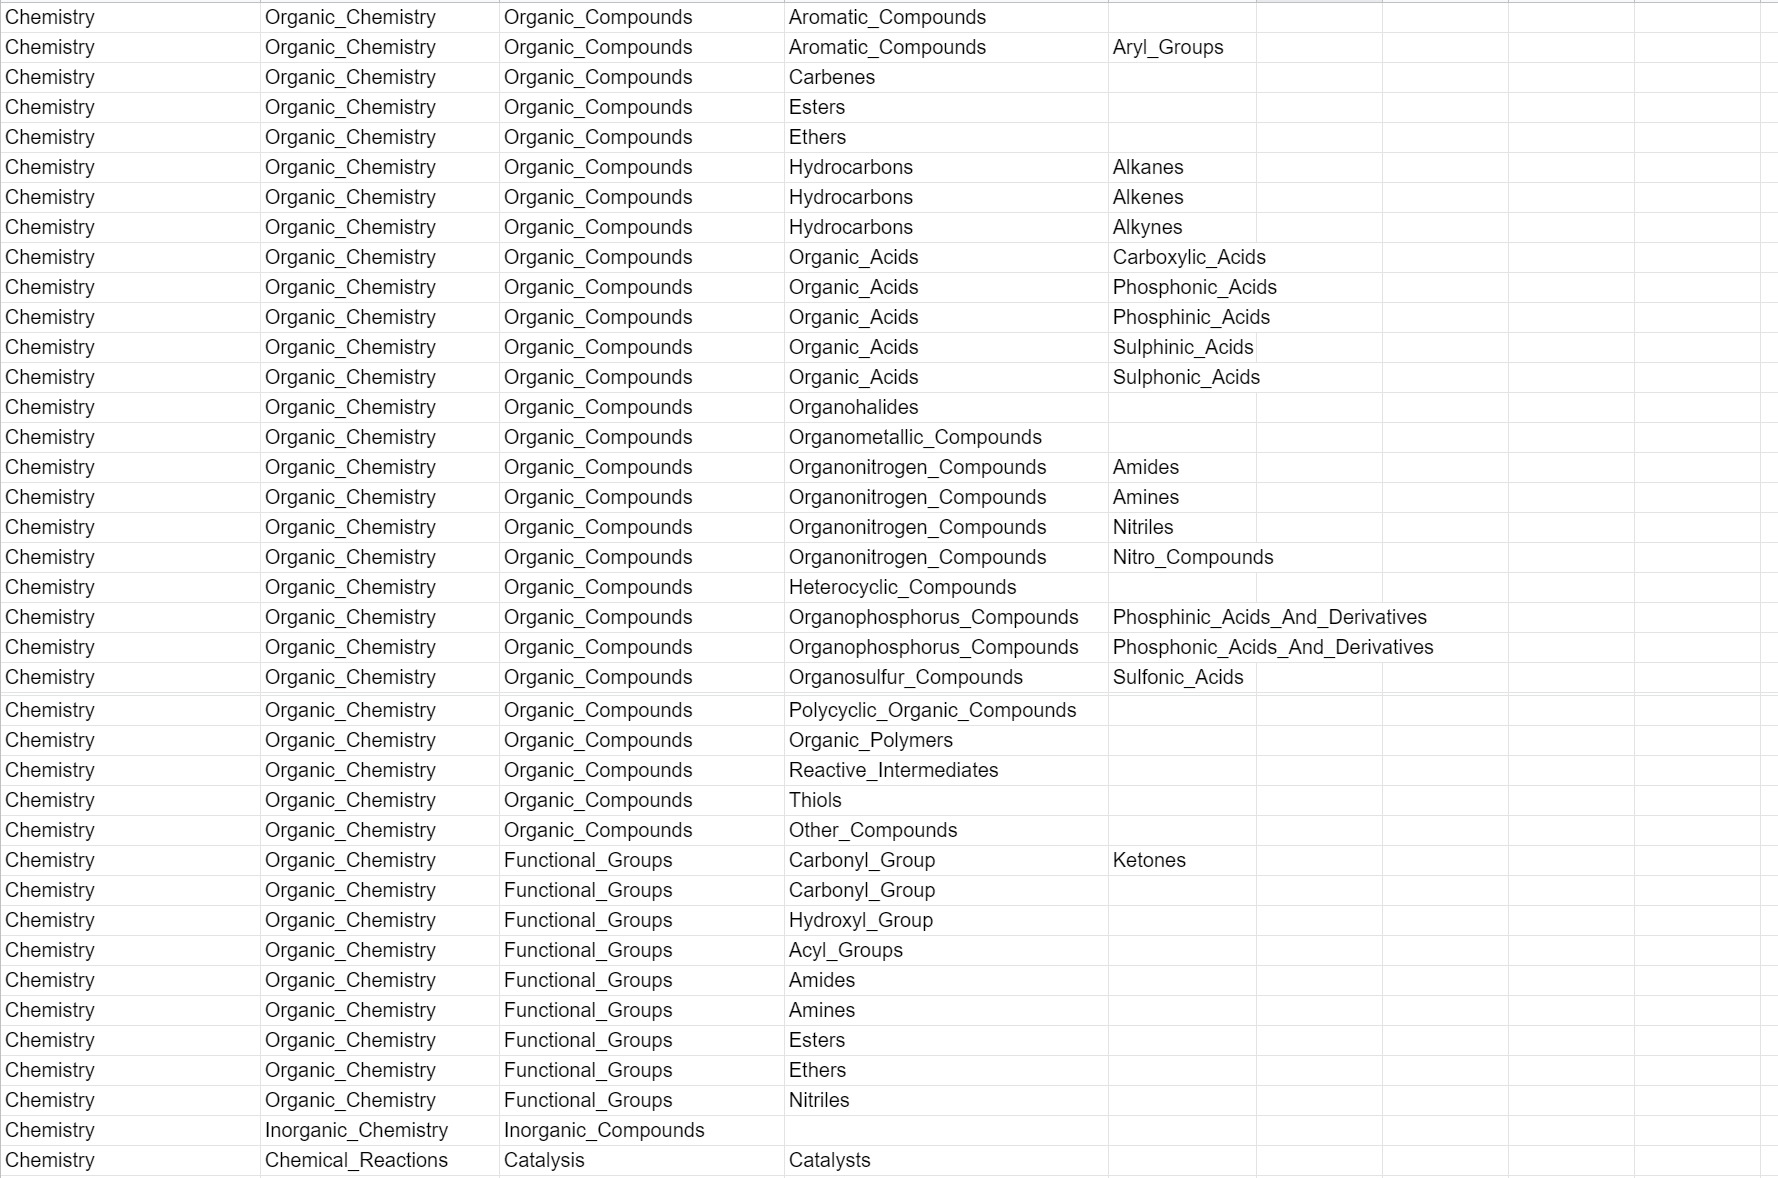
\includegraphics[width=2 
			\columnwidth]{ont.jpg}}
		\caption{Ontology Screenshot}
		\label{fig:ont}
	\end{center}
	% 	\vskip -0.2in
\end{figure*}



\end{document}
